\begin{flushright} {\tiny {\color{gray} (tikz\_chequerboard.tex)}} \end{flushright}
%~~~~~~~~~~~~~~~~~~~~~~~~~~~~~~~~~~~~~~~~~~~~~~~~~~~~~~~~~~~~~~~~~~~~~~~~~~~~~~~~~~~~~~~~~~~~~~~~~~

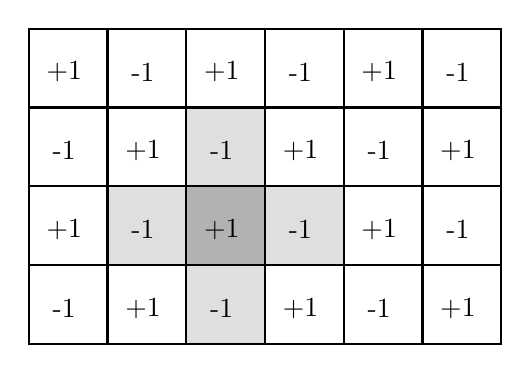
\begin{tikzpicture}
%\draw[step=0.5cm,gray,very thin] (0,0) grid (6,4); %background grid

\draw[fill=gray!60,gray!60](2,1) rectangle (3,2);
\draw[fill=gray!25,gray!25](2,0) rectangle (3,1);
\draw[fill=gray!25,gray!25](2,2) rectangle (3,3);
\draw[fill=gray!25,gray!25](1,1) rectangle (2,2);
\draw[fill=gray!25,gray!25](3,1) rectangle (4,2);

\draw[thick] (0,0)--(6,0)--(6,4)--(0,4)--cycle;  

\draw[thick] (0,1)--(6,1);  
\draw[thick] (0,2)--(6,2);  
\draw[thick] (0,3)--(6,3);  

\draw[thick] (1,0)--(1,4);  
\draw[thick] (2,0)--(2,4);  
\draw[thick] (3,0)--(3,4);  
\draw[thick] (4,0)--(4,4);  
\draw[thick] (5,0)--(5,4);  

\node[] at (0.45,0.45) {-1};
\node[] at (1.45,0.45) {+1};
\node[] at (2.45,0.45) {-1};
\node[] at (3.45,0.45) {+1};
\node[] at (4.45,0.45) {-1};
\node[] at (5.45,0.45) {+1};

\node[] at (0.45,1.45) {+1};
\node[] at (1.45,1.45) {-1};
\node[] at (2.45,1.45) {+1};
\node[] at (3.45,1.45) {-1};
\node[] at (4.45,1.45) {+1};
\node[] at (5.45,1.45) {-1};

\node[] at (0.45,2.45) {-1};
\node[] at (1.45,2.45) {+1};
\node[] at (2.45,2.45) {-1};
\node[] at (3.45,2.45) {+1};
\node[] at (4.45,2.45) {-1};
\node[] at (5.45,2.45) {+1};

\node[] at (0.45,3.45) {+1};
\node[] at (1.45,3.45) {-1};
\node[] at (2.45,3.45) {+1};
\node[] at (3.45,3.45) {-1};
\node[] at (4.45,3.45) {+1};
\node[] at (5.45,3.45) {-1};

\end{tikzpicture}


